\section{Experiments}

We evaluate our multitasking approach with in- and out-of-domain resources. We start by reporting results of models trained using only the Multi30K dataset. We also report the results of training the {\sc imaginet} decoder with the COCO dataset. Finally, we report results on incorporating the external News Commentary parallel text into our model. Throughout, we report performance of the  En$\rightarrow$De translation using Meteor \citep{denkowski:lavie:meteor-wmt:2014} and BLEU \citep{Papineni:2002:BMA:1073083.1073135} against lowercased tokenized references.

\subsection{Hyperparameters}

The encoder is a 1000D Gated Recurrent Unit bidirectional recurrent neural network \citep[GRU]{Cho2014} with 620D embeddings. We share all of the encoder parameters between the primary and auxiliary task. The translation decoder is a 1000D GRU recurrent neural network, with a 2000D context vector over the encoder states, and 620D word embeddings \citep{Sennrich2017}. The Imaginet decoder is a single-layer feed-forward network, where we learn the parameters $\mathbf{W_{vis}} \in \mathbb{R}^{2048\text{x}2000}$ to predict the true image vector with $\alpha = 0.1$ for the Imaginet objective (Equation \ref{eqn:imaginet}). The models are trained using the Adam optimiser with the default hyperparameters \citep{kingma2014adam} in minibatches of 80 instances. The translation task is defined as the primary task and convergence is reached when BLEU has not increased for five epochs on the validation data. Gradients are clipped when their norm exceeds 1.0. Dropout is set to 0.2 for the embeddings and the recurrent connections in both tasks \citep{Gal2016}. Translations are decoded using beam search with 12 hypotheses.

\subsection{In-domain experiments}\label{sec:in_domain_all}

% \begin{table}
% \centering
% \renewcommand{\arraystretch}{1.3}
% \begin{tabular}{lccc}
% \toprule
% & Meteor & BLEU \\
% \midrule
% \citep{toyama2016neural} & 50.6  & 34.5 \\
% Moses & 56.9 & 36.9\\
% NMT & 53.0 & 36.1 $\pm$ 1.2\\
% \citep{Calixto2017c} & 55.0 & 36.5 \\
% Ours & 55.8 & 38.4 $\pm$ 0.2\\
% \bottomrule
% \end{tabular}
% \caption{En$\rightarrow$De translation results on the Multi30K dataset. Our Multitask model is strong as a single model and sets a new state of the art as an ensemble. We report the mean and standard deviation of three random initialisations; the other results are taken from the literature.}\label{tab:results:in-domain}
% \end{table}

\begin{table}
\centering
\renewcommand{\arraystretch}{1.3}
\begin{tabular}{lccc}
\cmidrule[0.08em](l{5pt}r{5pt}){1-3}
& Meteor & BLEU \\
\cmidrule(l{5pt}r{5pt}){1-3}
NMT & 54.0 $\pm$ 0.6 & 35.5 $\pm$ 0.8\\
\cite{Calixto2017c} & 55.0 & 36.5 \\
\cite{Calixto2017b} & 55.1 & 37.3 \\
Imagination & 55.8 $\pm$ 0.4 & 36.8 $\pm$ 0.8\\
\cite{toyama2016neural} & 56.0  & 36.5 \\
\cite{Hitschler2016} & 56.1 & 34.3 \\
Moses & 56.9 & 36.9\\
\cmidrule[0.08em](l{5pt}r{5pt}){1-3}
\end{tabular}
\caption{En$\rightarrow$De translation results on the Multi30K dataset. Our Imagination model is competitive with the state of the art when it is trained on in-domain data. We report the mean and standard deviation of three random initialisations.}
\label{tab:results:in-domain}
\end{table}

We start by presenting the results of our multitask
model trained using only the Multi30K dataset. We compare against state-of-the-art approaches and text-only baselines. Moses is the phrase-based machine translation model \citep{Koehn2007} reported in \cite{Specia2016}. NMT is a text-only neural machine translation model.
\cite{Calixto2017c} is a double-attention model over the source language and the image.
\cite{Calixto2017b} is a multimodal translation model that conditions the decoder on semantic image vector extracted from the VGG-19 CNN.
\cite{Hitschler2016} uses visual features in a target-side retrieval model for translation. \cite{toyama2016neural} is most comparable to our approach: it is a multimodal variational NMT model that infers latent variables to represent the source language semantics from the image and linguistic data.

Table \ref{tab:results:in-domain} shows the results of this experiment.
We can see that the combination of the attention-based translation model and the image
prediction model is a 1.8 Meteor point improvement over the NMT
baseline, but it is 1.1 Meteor points worse than the strong Moses baseline. Our approach is competitive with previous approaches that use visual features as inputs to the decoder and the target-side reranking model. It also competitive with \cite{toyama2016neural}, which also only uses images for training.  These results confirm that our multitasking approach uses the image prediction task to improve the encoder of the translation model.

\begin{table}[t]
\centering
\renewcommand{\arraystretch}{1.3}
\begin{tabular}{lcc}
\cmidrule[0.08em](l{5pt}r{5pt}){1-3}
& Meteor & BLEU \\
\cmidrule(l{5pt}r{5pt}){1-3}
Imagination & 55.8 $\pm$ 0.4 & 36.8 $\pm$ 0.8 \\
Imagination (COCO) & 55.6 $\pm$ 0.5 & 36.4 $\pm$ 1.2 \\
\cmidrule[0.08em](l{5pt}r{5pt}){1-3}
\end{tabular}
\caption{Translation results when using out-of-domain described images. Our approach is still effective when the image prediction model is trained over the COCO dataset.}\label{tab:results:ood-coco}
\end{table}

\subsection{External described image data}\label{sec:experiments:ood-images}


\begin{table}
\centering
\renewcommand{\arraystretch}{1.3}
\begin{tabular}{@{}lcc}
\cmidrule[0.08em](l{1pt}r{5pt}){1-3}
 & Meteor & BLEU \\
\cmidrule(l{1pt}r{5pt}){1-3}
NMT & 52.8 $\pm$ 0.6 & 33.4 $\pm$ 0.6\\
+ NC & 56.7 $\pm$ 0.3 & 37.2 $\pm$ 0.7 \\
+ Imagination & 56.7 $\pm$ 0.1 & 37.4 $\pm$ 0.3 \\
+ Imagination (COCO) & 57.1 $\pm$ 0.2 & 37.8 $\pm$ 0.7 \\
\cite{Calixto2017c} & 56.8 & 39.0 \\
\cmidrule[0.08em](l{1pt}r{5pt}){1-3}
\end{tabular}
	\caption{Translation results with out-of-domain parallel text and described images. We find further improvements when we multitask with the News Commentary (NC) and COCO datasets.}\label{tab:results:ood-both}
\end{table}

Recall from Section \ref{sec:problem} that we are interested in scenarios where $x$, $y$, and $v$ are drawn from different sources. We now experiment with separating the translation data from the described image data using $\mathcal{D}_{image}$: MS COCO dataset of 83K described images\footnote{Due to differences in the vocabularies of the respective datasets, we do not train on examples where more than 10\% of the tokens are out-of-vocabulary in the Multi30K dataset.} and $\mathcal{D}_{text}$: Multi30K parallel text.

Table \ref{tab:results:ood-coco} shows the results of this experiment.
We find that there is no significant difference between training the {\sc imaginet} decoder on in-domain (Multi30K) or out-of-domain data (COCO). This result confirms that we can separate the parallel text from the described images.

\subsection{External parallel text data}

% \begin{table}[t]
% \centering
% 	\begin{tabular}{ccccccc}
%     \cmidrule(r){1-7}
%     & \multicolumn{2}{c}{Bitext} & \multicolumn{2}{c}{Images} \\
%     & 30K & NC & 30K & COCO &  Meteor & {\small BLEU}\\
%     \cmidrule(r){1-7}
%     \parbox[t]{2mm}{\multirow{3}{*}{\rotatebox[origin=c]{90}{Zmorge}}} & \checkmark   &   &   &       & 56.2   & 37.8 \\[2.5ex]
%     & \checkmark   &   &  \checkmark  &           & 57.6   & 39.0 \\
%     \cmidrule(r){1-7}
%     \parbox[t]{2mm}{\multirow{4}{*}{\rotatebox[origin=c]{90}{Sub-word}}} & \checkmark   &   &   &       & 54.4   & 35.0 \\
% 	& \checkmark   &   \checkmark    &   &               & 58.6   & 39.4 \\
%     & \checkmark   & \checkmark  & \checkmark   &   & 59.0   & 39.5 \\
%     & \checkmark   &  \checkmark &   &   \checkmark      & \textbf{59.3}   & \textbf{40.2} \\
% \cmidrule(r){1-7}
% \end{tabular}
%     \caption{Ensemble decoding results. Zmorge denotes models trained with decompounded German words; Sub-word denotes joint SentencePiece word splitting (see Section \ref{sec:data} for more details).}\label{tab:results:ensemble}
% \end{table}

\begin{table*}[t]
\centering
        \begin{tabular}{ccccccc}
    \toprule
    & \multicolumn{2}{c}{Parallel text} & \multicolumn{2}{c}{Described images} \\
    & Multi30K & News Commentary & Multi30K & COCO & Meteor & BLEU \\
    \midrule
    \parbox[t]{2mm}{\multirow{3}{*}{\rotatebox[origin=c]{90}{Zmorge}}} & \checkmark   &   &   &       & 56.2   & 37.8 \\[2.5ex]
    & \checkmark   &   &  \checkmark  &           & 57.6   & 39.0 \\
    \midrule
    \parbox[t]{2mm}{\multirow{4}{*}{\rotatebox[origin=c]{90}{Sub-word}}} & \checkmark   &   &   &       & 54.4   & 35.0 \\
        & \checkmark   &   \checkmark    &   &               & 58.6   & 39.4 \\
    & \checkmark   & \checkmark  & \checkmark   &   & 59.0   & 39.5 \\
    & \checkmark   &  \checkmark &   &   \checkmark      & \textbf{59.3}   & \textbf{40.2} \\
\bottomrule
\end{tabular}
    \caption{Ensemble decoding results. Zmorge denotes models trained with decompounded German words; Sub-word denotes joint SentencePiece word splitting (see Section \ref{sec:data} for more details).}\label{tab:results:ensemble}
\end{table*}


We now experiment with training our model on a combination of the Multi30K and the News Commentary English-German data. In these experiments, we concatenate the Multi30K and News Commentary datasets into a single $\mathcal{D}_{text}$ training dataset, similar to \cite{Freitag2016}. We compare our model against \cite{Calixto2017c}, who pre-train their model on the WMT'15 English-German parallel text and back-translate \citep{Sennrich2016b} additional sentences from the bilingual independent descriptions in the Multi30K dataset (Footnote 2).

%\footnote{We tried creating an additional auxiliary task for the external data but the model underfits the external data before training converges on the Multi30K dataset.}

Table \ref{tab:results:ood-both} presents the results. The text-only NMT model using sub-words is 1.2 Meteor points lower than decompounding the German text. Nevertheless, the model trained over a concatenation of the parallel texts is a 2.7 Meteor point improvement over this baseline (+ NC) and matches the performance of our Multitasking model that uses only in-domain data (Section \ref{sec:in_domain_all}). We do not see an additive improvement for the multitasking model with the concatenated parallel text and the in-domain data (+ Imagination) using a training objective interpolation of $w = 0.89$ (the ratio of the training dataset sizes). This may be because we are essentially learning a translation model and the updates from the {\sc imaginet} decoder are forgotten. Therefore, we experiment with multitasking the concatenated parallel text and the COCO dataset ($w=0.5$). We find that balancing the datasets improves over the concatenated text model by 0.4 Meteor (+ Imagination (COCO)). Our multitasking approach improves upon Calixto et al. by 0.3 Meteor points. Our model can be trained in 48 hours using 240K parallel sentences and 414K described images from out-of-domain datasets. Furthermore, recall that our model does not use images as an input for translating unseen data, which results in 6.2\% fewer parameters compared to using the 2048D Inception-V3 visual features to initialise the hidden state of the decoder.

\begin{table*}[h]
\renewcommand{\arraystretch}{1.2}
\begin{subtable}{0.22\textwidth}
\centering
\begin{tabular}{c}
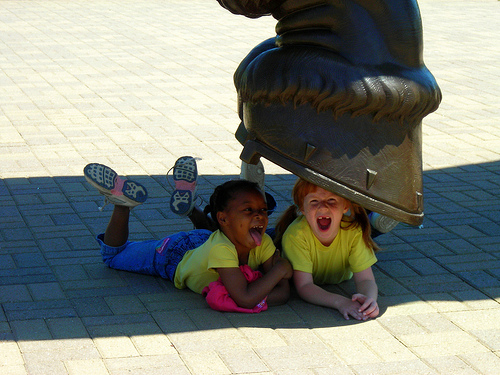
\includegraphics[width=0.7\textwidth]{chapters/IJCNLP/images/533602654.jpg}
\end{tabular}
\end{subtable}%
\begin{subtable}{0.75\textwidth}
\begin{tabular}{rp{27em}}
Source: & two children on their stomachs lay on the ground under a pipe \\
NMT: & zwei kinder \textcolor{red}{auf ihren gesichtern} liegen unter dem boden auf dem boden \\
Ours: & zwei kinder liegen bäuchlings auf dem boden unter einer \textcolor{red}{schaukel}
 \\
\end{tabular}
\end{subtable}

\vspace{0em}

\begin{subtable}{0.22\textwidth}
\centering
\begin{tabular}{c}
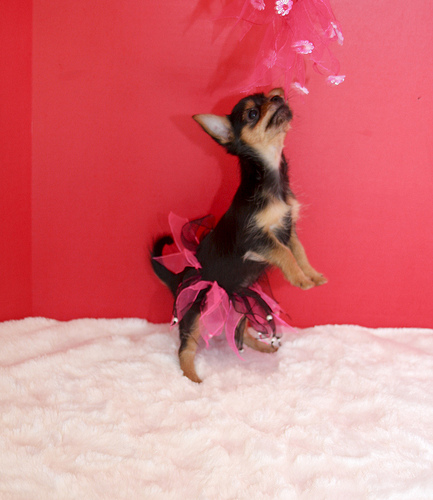
\includegraphics[width=0.7\textwidth]{chapters/IJCNLP/images/3720366614.jpg}
\end{tabular}
\end{subtable}%
\begin{subtable}{0.75\textwidth}
\begin{tabular}{rp{27em}}
Source: & small dog in costume stands on hind legs to reach dangling flowers \\
NMT: & ein kleiner hund steht auf dem hinterbeinen und \textcolor{red}{läuft} , \textcolor{red}{nach links von blumen zu sehen}  \\
Ours: & ein kleiner hund in einem kostüm steht auf den hinterbeinen , um die blumen zu erreichen\\
\end{tabular}

\end{subtable}

\vspace{0em}

\begin{subtable}{0.22\textwidth}
\centering
\begin{tabular}{c}
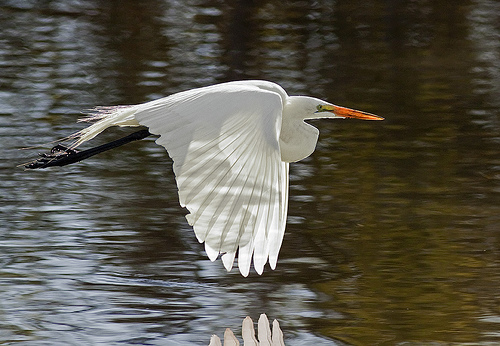
\includegraphics[width=0.7\textwidth]{chapters/IJCNLP/images/3325578605.jpg}
\end{tabular}
\end{subtable}%
\begin{subtable}{0.75\textwidth}
\begin{tabular}{rp{27em}}
Source: & a bird flies across the water \\
NMT: & ein vogel fliegt über das wasser \\
Ours: & ein vogel fliegt \textcolor{red}{durch} das wasser\\
\end{tabular}
\end{subtable}

\caption{Examples where our model improves or worsens the translation compared to the NMT baseline. Top: NMT translates the wrong body part; both models skip ``pipe''. Middle: NMT incorrectly translates the verb and misses several nouns. Bottom: Our model incorrectly translates the preposition.}\label{tab:results:examples}
\end{table*}


\subsection{Ensemble results}

Table \ref{tab:results:ensemble} presents the results of ensembling different randomly initialised models. We achieve a start-of-the-art result of 57.6 Meteor for a model trained on only in-domain data. The improvements are more pronounced for the models trained using sub-words and out-of-domain data. An ensemble of baselines trained on sub-words is initially worse than an ensemble trained on Zmorge decompounded words. However, we always see an improvement from ensembling models trained on in- and out-of-domain data. Our best ensemble is trained on Multi30K parallel text, the News Commentary parallel text, and the COCO descriptions to set a new state-of-the-art result of 59.3 Meteor.

\subsection{Multi30K 2017 results}

We also evaluate our approach against 16 submissions to the WMT Shared Task on Multimodal Translation and Multilingual Image Description \citep{elliott2017imagination}. This shared task features a new evaluation dataset: Multi30K Test 2017 \citep{elliott2017imagination}, which contains 1,000 new evaluation images. The shared task submissions are evaluated with Meteor and human direct assessment \citep{Graham2017}. We submitted two systems, based on whether they used only the Multi30K dataset (constrained) or used additional external resources (unconstrained). Our constrained submission is an ensemble of three Imagination models trained over only the Multi30K training data. This achieves a Meteor score of 51.2, and a joint 3rd place ranking according to human assessment. Our unconstrained submission is an ensemble of three Imagination models trained with the Multi30K, News Commentary, and MS COCO datasets. It achieves a Meteor score of 53.5, and 2nd place in the human assessment.

\subsection{Qualitative examples}

Table \ref{tab:results:examples} shows examples of where the multitasking model improves or worsens translation performance compared to the baseline model\footnote{We used MT-ComparEval \citep{Klejch2015}}. The first example shows that the baseline model makes a significant error in translating the pose of the children, translating ``on their stomachs'' as ``on their faces''). The middle example demonstrates that the baseline model translates the dog as walking (``läuft'') and then makes grammatical and sense errors after the clause marker. Both models neglect to translate the word ``dangling'', which is a low-frequency word in the training data. There are instances where the baseline produces better translations than the multitask model: In the bottom example, our model translates a bird flying through the water (``durch'') instead of ``over'' the water.
